\begin{definition} Se define el  espacio $\mathbb{R}^n$  como el conjunto formado por todas las $n$-uplas de n\'umeros reales ordenados.   Es decir:
    \begin{equation*}
        \mathbb{R}^n = \left\{ \boldsymbol{v} / \boldsymbol{v}=(x_1,x_2,x_3,...,x_n), \; x_i \in \mathbb{R} \;\forall \;   1\leq  i \leq n  \right\}
    \end{equation*}
\end{definition}

\begin{definition}  Sean  $\mathbb{V}$ y $\mathbb{W}$ sub-espacios vectoriales de $\mathbb{R}^n$.  Se  define a  una transformación lineal  como a  una función 
    \begin{equation*}
       \boldsymbol{T}: \mathbb{V} \rightarrow  \mathbb{W}
    \end{equation*}
    que cumple con la condición de linealidad:
    \begin{equation}\label{tl}
        \boldsymbol{T}(\alpha \cdot \boldsymbol{v_1} + \beta \cdot \boldsymbol{v_2})=\alpha \cdot \boldsymbol{T}(\boldsymbol{v_2}) + \beta \cdot \boldsymbol{T}(\boldsymbol{v_2}),
    \end{equation}
    donde $\boldsymbol{v_1},\boldsymbol{v_2} \in \mathbb{V}$ y $\alpha,\beta \in \mathbb{R}$. 
    \label{def:TL}
\end{definition}



\begin{definition} Sean    $\boldsymbol{v}\in\mathbb{R}^n$   no nulo y  $\boldsymbol{x_0}\in\mathbb{R}^n,$  el conjunto $L \subset \mathbb{R}^n $  que cumple  
 \begin{equation*}
      L = \{   \boldsymbol{x} \in\mathbb{R}^n  \:| \:    \boldsymbol{x}=  \lambda \cdot \boldsymbol{v} + \boldsymbol{x_0},  \:  \mbox{  con }  \lambda\in\mathbb{R} \}.
    \end{equation*}  es una recta en $ \mathbb{R}^n $  y a la ecuaci\'on $$ \boldsymbol{x}=  \lambda \cdot \boldsymbol{v} + \boldsymbol{x_0}$$  se  llama  \textbf{expresi\'on vectorial} de la misma.  
    Adem\'as, llamaremos al vector $\boldsymbol{x_0}$ como \textbf{vector posici\'on} (o punto de paso) de la recta y al vector $\boldsymbol{v}$ como \textbf{vector director} de la recta.
 \end{definition}

 \begin{figure}[H]
 \begin{center}
  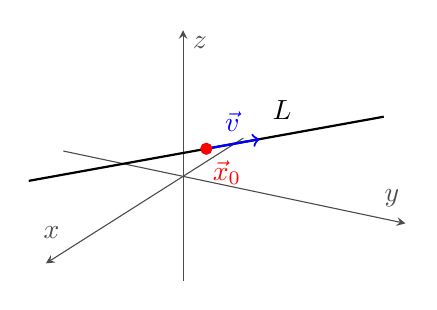
\begin{tikzpicture}
    \begin{axis}[
      view={120}{30},
      axis lines=middle,
      axis line style={black!70},
      label style={black!70},
      enlargelimits=0.5,
      ticks=none,
      xlabel={$x$}, ylabel={$y$}, zlabel={$z$},
      xmin=-1, xmax=8,
      ymin=-1, ymax=4,
      zmin=-1, zmax=2,
    ]
  
      % Punto de paso x_0
      \addplot3[only marks, color=red, mark=*] coordinates {(1, 1, 1)};
      \node at (axis cs:1.3,1.7,0.6) {$\textcolor{red}{\vec{x}_0}$};
  
     
  
      % Recta L: r(t) = x_0 + t * v
      \addplot3[
        domain=-10:10,
        samples=50,
        samples y=0,
        thick,
        black,
        variable=t,
        parametric,
      ] 
      ({1 + 1.5*t}, {1 + 1*t}, {1 + 0.5*t});
      \node at (axis cs:5,4.5,3.2) {$L$};
  
       % Vector director v (desde x_0)
      \addplot3[->, thick, blue] coordinates {(1,1,1) (5.5,4,2.5)};
      \node at (axis cs:3.3,2.5,2.3) {$\textcolor{blue}{\vec{v}}$};
  
    \end{axis}
  \end{tikzpicture}
  \caption{Ejemplo de una recta $L$, con su vector director $\vect{v}$ y punto de paso $\vect{x_0}$.}
  \end{center}
\end{figure}

\begin{definition} Sean    $\boldsymbol{n}\in\mathbb{R}^3$   no nulo  y  $\boldsymbol{x_0}\in\mathbb{R}^3,$  el conjunto $\pi \subset \mathbb{R}^3 $  que cumple  
    \begin{equation*}
      \pi  = \{   \boldsymbol{x} \in\mathbb{R}^3  \:| \:    \boldsymbol{n}\cdot(\boldsymbol{x} - \boldsymbol{x_0}) =0   \}.
    \end{equation*} es un plano en $\mathbb{R}^3$  y a la ecuaci\'on   $$ \boldsymbol{n}\cdot(\boldsymbol{x} - \boldsymbol{x_0}) =0$$  se llama  \textbf{expresi\'on canónica} del mismo.  Adem\'as, llamaremos al vector $\boldsymbol{n}$   como \textbf{vector normal} del plano 
    y al vector  $\boldsymbol{x_0}$ \textbf{punto de paso} del plano. 

    A su vez, también se puede expresar un plano análogamente a la forma propuesta para la recta:
    \begin{equation*}
      \pi  = \{   \boldsymbol{x} \in\mathbb{R}^3  \:| \:    \boldsymbol{x}=\boldsymbol{x_0}+\alpha \boldsymbol{u} + \beta \boldsymbol{u},  \:  \mbox{  con }  \alpha,\beta\in\mathbb{R}    \}.
    \end{equation*} tal que la ecuación
    \begin{equation*}
       \boldsymbol{x}=\boldsymbol{x_0}+\alpha \boldsymbol{u} + \beta \boldsymbol{v}
    \end{equation*}
    se conoce como la \textbf{forma vectorial} del plano. Donde $\boldsymbol{u}$ y $\boldsymbol{v}$ son dos \textbf{vectores paralelos al plano}, que cumplen que $\boldsymbol{v}\times\boldsymbol{u}\shortparallel \boldsymbol{n}$, el vector normal del plano.
    Finalmente, $\alpha$ y $\beta$ son \textbf{parámetros} reales.

 \end{definition}
   
 \begin{figure}[H]
  \begin{center}
    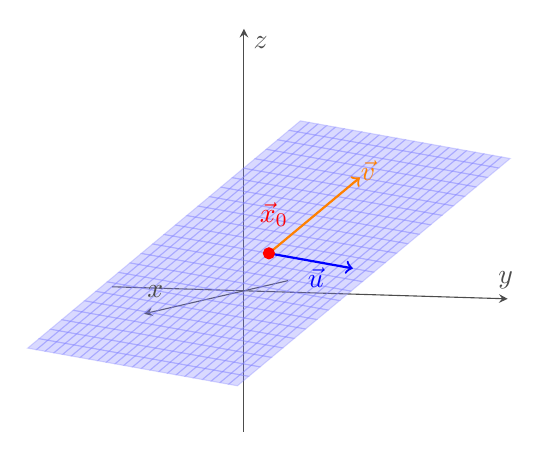
\begin{tikzpicture}
      \begin{axis}[
        view={110}{5},
        axis lines=middle,
        axis line style={black!70},
        label style={black!70},
        enlargelimits=0.5,
        ticks=none,
        xlabel={$x$}, ylabel={$y$}, zlabel={$z$},
        xmin=-1, xmax=8,
        ymin=-1, ymax=5,
        zmin=-1, zmax=4,
      ]
    
        
    
        % Plano generado por x_0 + s*u + t*v
        \addplot3[
          surf,
          opacity=0.3,
          color=blue!50!white,
          shader=flat,
          domain=-5:5,
          domain y=-1.5:1.5,
        ]
        (
          {1 + 1.5*x + 1*y},
          {1 + 1*x + 3*y},
          {1 + 0*x + 2*y}
        );
    
        % Punto de paso x_0
        \addplot3[only marks, color=red, mark=*] coordinates {(1, 1, 1)};
        \node at (axis cs:1.6,1.3,2) {$\textcolor{red}{\vec{x}_0}$};
    
        % Vectores u y v
        \addplot3[->, thick, blue] coordinates {(1,1,1) (7,5,1)};
        \node at (axis cs:4.2,3.2,0.6) {$\textcolor{blue}{\vec{u}}$};
    
        \addplot3[->, thick, orange] coordinates {(1,1,1) (2,4,3)};
        \node at (axis cs:2.2,4.3,3.2) {$\textcolor{orange}{\vec{v}}$};
    
      \end{axis}
    \end{tikzpicture}
   \caption{Ejemplo un plano $\pi$, con su punto de paso $\vect{x_0}$ y vector normal $\vect{n}$.}
   \end{center}
 \end{figure}

 \begin{figure}[H]
  \begin{center}
    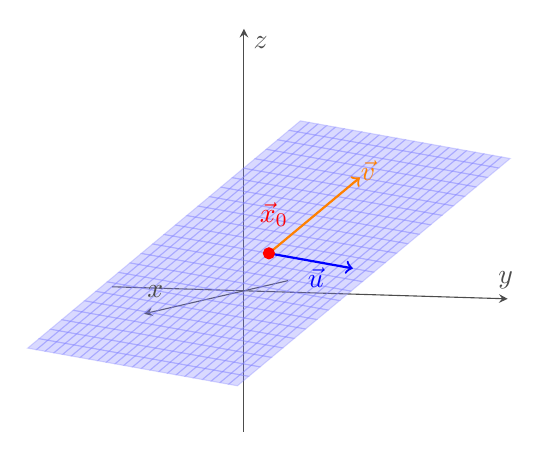
\begin{tikzpicture}
      \begin{axis}[
        view={110}{5},
        axis lines=middle,
        axis line style={black!70},
        label style={black!70},
        enlargelimits=0.5,
        ticks=none,
        xlabel={$x$}, ylabel={$y$}, zlabel={$z$},
        xmin=-1, xmax=8,
        ymin=-1, ymax=5,
        zmin=-1, zmax=4,
      ]
    
        
    
        % Plano generado por x_0 + s*u + t*v
        \addplot3[
          surf,
          opacity=0.3,
          color=blue!50!white,
          shader=flat,
          domain=-5:5,
          domain y=-1.5:1.5,
        ]
        (
          {1 + 1.5*x + 1*y},
          {1 + 1*x + 3*y},
          {1 + 0*x + 2*y}
        );
    
        % Punto de paso x_0
        \addplot3[only marks, color=red, mark=*] coordinates {(1, 1, 1)};
        \node at (axis cs:1.6,1.3,2) {$\textcolor{red}{\vec{x}_0}$};
    
        % Vectores u y v
        \addplot3[->, thick, blue] coordinates {(1,1,1) (7,5,1)};
        \node at (axis cs:4.2,3.2,0.6) {$\textcolor{blue}{\vec{u}}$};
    
        \addplot3[->, thick, orange] coordinates {(1,1,1) (2,4,3)};
        \node at (axis cs:2.2,4.3,3.2) {$\textcolor{orange}{\vec{v}}$};
    
      \end{axis}
    \end{tikzpicture}
   \caption{Ejemplo del mismo plano de la figura anterior, $\pi$, pero con sus vectores directores $\vect{v}$ y $\vect{u}$ y punto de paso $\vect{x_0}$.}
   \end{center}
 \end{figure}


   
  %\textcolor{red}{Agregar forma vectorial del plano}

  
  

\begin{definition} Sean  $(x_0,y_0) \in \mathbb{R}^2$ y $r \in \mathbb{R}_{ > 0}. $

  El conjunto $C \subset \mathbb{R}^2$ que cumple
    \begin{equation*}\label{circ}
    C = \{  (x,y)  \in \mathbb{R}^2 \:|\:   (x-x_0)^2+(y-y_0)^2=r^2 \}
    \end{equation*}  es una circunferencia en el plano. Adem\'as, al vector $(x_0,y_0)$  se lo llama centro y al n\'umero $r$  se lo llama radio de la misma.
   
  El conjunto $D \subset \mathbb{R}^2$ que cumple
    \begin{equation*}
    D = \{  (x,y)  \in \mathbb{R}^2 \:|\:   (x-x_0)^2+(y-y_0)^2 \leq r^2 \}
    \end{equation*}  es un c\'irculo en el plano. Adem\'as, al vector $(x_0,y_0)$  se lo llama centro y al n\'umero $r$  se lo llama radio del mismo.  
   \end{definition}
   \begin{figure}[H]
    \begin{center}
      \begin{tikzpicture}
        \begin{axis}[
          axis lines=middle,
          axis line style={black!70},
          label style={black!70},
          ticks=none,
          xlabel={$x$}, ylabel={$y$},
          xmin=-1, xmax=4,
          ymin=-1, ymax=4,
          width=10cm,
          height=10cm,
        ]
      
          % Centro de la circunferencia
          \def\xo{2}
          \def\yo{2}
          \def\radio{1.5}
      
          % Circunferencia
          \addplot [
            domain=0:360,
            samples=200,
            smooth,
            thick,
            black
          ] ({\xo + \radio*cos(x)}, {\yo + \radio*sin(x)});
          
          % Etiqueta para la circunferencia
          \node at (axis cs:{\xo + \radio + 0.1}, {\yo+1}) {$C$};
      
          % Punto (x_0, y_0)
          \addplot[only marks, mark=*, red] coordinates {(\xo,\yo)};
          \node at (axis cs:{\xo + 0.4}, {\yo + 0.4}) {$\textcolor{red}{(x_0, y_0)}$};

          % Vector radio (desde el centro hacia la derecha)
          \addplot[->, thick, blue] coordinates {(\xo, \yo) ({\xo + \radio}, \yo)};
          \node at (axis cs:{\xo + \radio/2}, {\yo - 0.2}) {$\textcolor{blue}{r}$};
      
        \end{axis}
      \end{tikzpicture}
     \caption{Circunferencia $C$ de radio $r$ y centro $(x_0,y_0)$.}
     \end{center}
   \end{figure}
   
   \begin{figure}[H]
    \begin{center}
      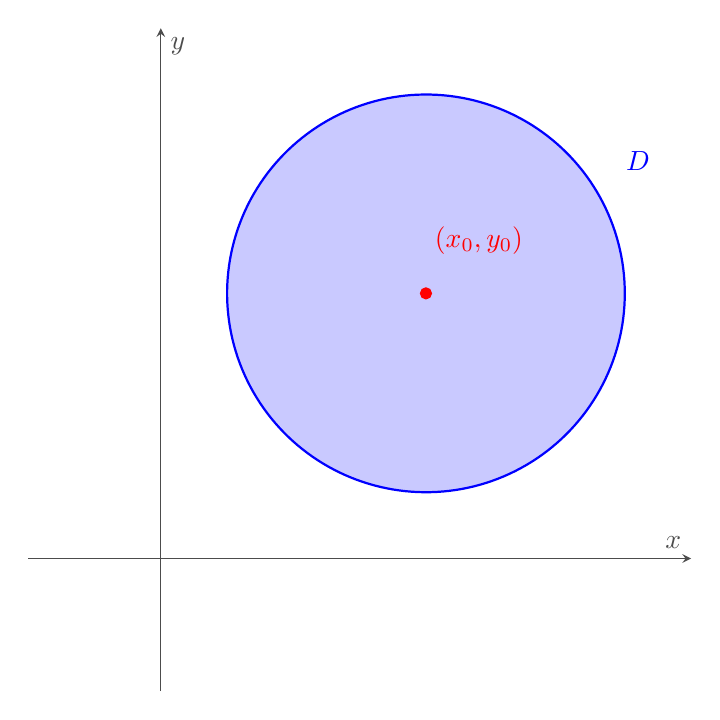
\begin{tikzpicture}
        \begin{axis}[
          axis lines=middle,
          axis line style={black!70},
          label style={black!70},
          ticks=none,
          xlabel={$x$}, ylabel={$y$},
          xmin=-1, xmax=4,
          ymin=-1, ymax=4,
          width=10cm,
          height=10cm,
        ]
      
          % Centro de la circunferencia
          \def\xo{2}
          \def\yo{2}
          \def\radio{1.5}
      
          % Circunferencia rellena
          \addplot [
            domain=0:360,
            samples=200,
            fill=blue!70,
            fill opacity=0.3,
            draw=blue,
            thick,
          ] ({\xo + \radio*cos(x)}, {\yo + \radio*sin(x)});
          
          % Etiqueta para la circunferencia
          \node at (axis cs:{\xo + \radio + 0.1}, {\yo+1}) {$\textcolor{blue}{D}$};
      
          % Punto (x_0, y_0)
          \addplot[only marks, mark=*, red] coordinates {(\xo,\yo)};
          \node at (axis cs:{\xo + 0.4}, {\yo + 0.4}) {$\textcolor{red}{(x_0, y_0)}$};
          
      
        \end{axis}
      \end{tikzpicture}
     \caption{Si se rellena la circunferencia $C$ se obtiene el circulo $D$. Es decir, el círculo $D$ de la figura tiene como borde, o frontera, la circunferencia $C$.}
     \end{center}
   \end{figure}
   
   
\begin{definition}\textbf{Ecuación de la esfera.}
    La cáscara de una esfera (es decir, sólo su superficie exterior, hueca) 
    se expresa como un conjunto $A\subset\mathbb{R}^3$ que cumple
    \begin{equation*}
      S = \{  (x,y,z)  \in \mathbb{R}^3 \:|\:   (x-x_0)^2+(y-y_0)^2+(z-z_0)^2=r^2 \}
    \end{equation*}
    Se tiene $(x_0,y_0,z_0)$ como el centro de la cáscara y $r$ como el radio de la misma.
    Para obtener un conjunto $B\subset\mathbb{R}^3$ que represente la esfera completa, es decir, cáscara y relleno interior, se debe tener
    \begin{equation*}
      V = \{  (x,y,z)  \in \mathbb{R}^3 \:|\:   (x-x_0)^2+(y-y_0)^2+(z-z_0)^2\leq r^2 \}
    \end{equation*}
    Esto es análogo al caso de la circunferencia y el círculo.
\end{definition}

\begin{figure}[H]
  \begin{center}
    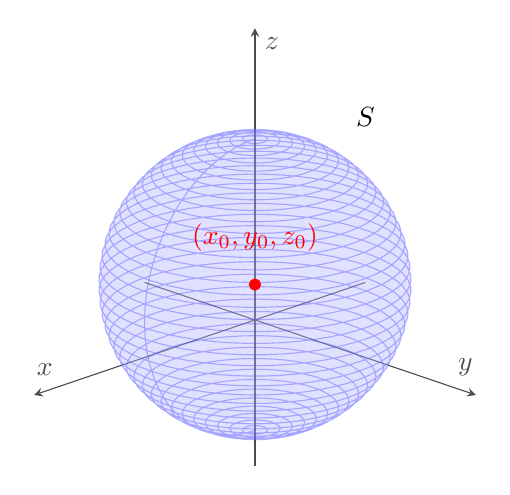
\begin{tikzpicture}
      \begin{axis}[
        view={135}{20},
        axis lines=middle,
        axis line style={black!70},
        label style={black!70},
        ticks=none,
        xlabel={$x$}, ylabel={$y$}, zlabel={$z$},
        xmin=-2, xmax=4,
        ymin=-2, ymax=4,
        zmin=-2, zmax=4,
        width=10cm,
        height=10cm,
      ]
    
        % Centro y radio
        \def\xo{1}
        \def\yo{1}
        \def\zo{1}
        \def\radio{2}
    
        % Esfera con borde visible
        \addplot3[
          domain=0:360,
          y domain=0:180,
          draw=blue!70,
          fill=blue!30,
          opacity=0.4,
          faceted color=blue!60,
          shader=flat,
          samples=60,
          samples y=40,
        ]
        (
          {\xo + \radio * cos(x) * sin(y)},
          {\yo + \radio * sin(x) * sin(y)},
          {\zo + \radio * cos(y)}
        );
    
        % Punto central
        \addplot3[only marks, color=red, mark=*] coordinates {(\xo,\yo,\zo)};
        \node at (axis cs:{\xo + 0.5},{\yo + 0.5},{\zo + 0.9}) {\textcolor{red}{\((x_0, y_0, z_0)\)}};
    
        % Etiqueta para la esfera
        \node at (axis cs:{\xo + \radio + 0.3},{\yo + \radio + 2.3},{\zo+4}) {$S$};
    
      \end{axis}
    \end{tikzpicture}
   \caption{Cáscara de esfera $S$ con centro $(x_0,y_0,z_0)$.}
   \end{center}
 \end{figure}

 \begin{figure}[H]
  \begin{center}
    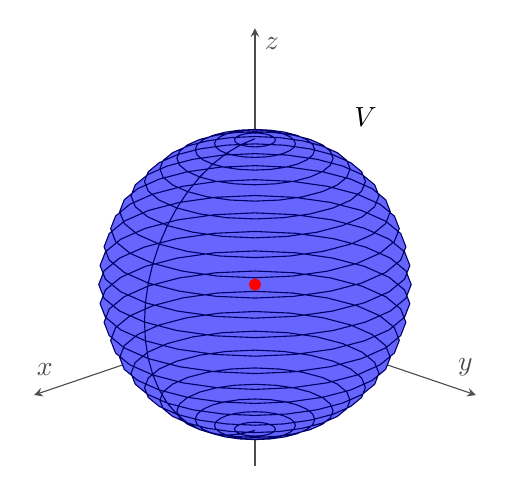
\begin{tikzpicture}
      \begin{axis}[
        view={135}{20},
        axis lines=middle,
        axis line style={black!70},
        label style={black!70},
        ticks=none,
        xlabel={$x$}, ylabel={$y$}, zlabel={$z$},
        xmin=-2, xmax=4,
        ymin=-2, ymax=4,
        zmin=-2, zmax=4,
        width=10cm,
        height=10cm,
      ]
    
        % Centro y radio
        \def\xo{1}
        \def\yo{1}
        \def\zo{1}
        \def\radio{2}
    
        % Esfera con borde visible
        \addplot3[
          faceted color=blue!60,
          draw=blue!40!black,             % sin líneas visibles
          fill=blue!60!white,
          opacity=1,
          shader=interp,
          domain=0:360,
          y domain=0:180,
        ]
        (
          {\xo + \radio * cos(x) * sin(y)},
          {\yo + \radio * sin(x) * sin(y)},
          {\zo + \radio * cos(y)}
        );
    
        % Punto central
        \addplot3[only marks, color=red, mark=*] coordinates {(\xo,\yo,\zo)};
        
    
        % Etiqueta para la esfera
        \node at (axis cs:{\xo + \radio + 0.3},{\yo + \radio + 2.3},{\zo+4}) {$V$};
    
      \end{axis}
    \end{tikzpicture}
   \caption{Esfera rellena $V$, que tiene como cáscara a $S$, de la figura anterior.}
   \end{center}
 \end{figure}
   